\documentclass[10pt]{article}
\usepackage[a4paper,margin=2cm]{geometry}
\usepackage[T1]{fontenc}
\usepackage{lmodern,microtype,booktabs,longtable,array,graphicx,caption,xcolor}
\captionsetup{font=small,labelfont=bf}
\renewcommand{\thetable}{S\arabic{table}}
\renewcommand{\thefigure}{S\arabic{figure}}
\title{Supplementary Materials\\[4pt]\large Cycle Time versus Accuracy: The Simulated Economic Value of\\AI-Based Phenotyping in Smallholder Bean Breeding}
\author{Juk-Sen Tang and Junhong Chen}
\date{}
\begin{document}
\maketitle
\vspace{-2em}
{\small\begin{longtable}{@{}>{\raggedright\arraybackslash}p{0.06\linewidth}>{\raggedright\arraybackslash}p{0.17\linewidth}>{\raggedright\arraybackslash}p{0.58\linewidth}r@{}}
\caption{Search queries for the three meta-analyses, run on 5 October 2026. Federated search: one query sent to OpenAlex, Semantic Scholar and Crossref, which returned at most 25 records per query and source. Hits: records returned; failed: no usable response.}\label{tab:S1}\\
\toprule ID & Source & Query & Hits\\ \midrule \endfirsthead
\toprule ID & Source & Query & Hits\\ \midrule \endhead
\bottomrule \endfoot
\multicolumn{4}{l}{\textbf{MA1 Realized genetic gain}}\\
q1 & Federated search & genetic gain common bean Phaseolus vulgaris grain yield breeding program & 25\\
q2 & Federated search & genetic progress common bean yield historical trials & 20\\
q3 & Federated search & genetic gain Phaseolus vulgaris era trial old new cultivars yield & 25\\
q4 & Federated search & realized genetic gain common bean Africa & 20\\
q5 & Federated search & genetic gain cowpea grain yield breeding & 23\\
q6 & Federated search & genetic gain soybean Africa Brazil era study yield & 25\\
q7 & Federated search & genetic gain groundnut peanut breeding yield historical & 25\\
q8 & Federated search & genetic gain chickpea yield breeding & 20\\
q9 & Federated search & genetic gain dry bean breeding yield Michigan OR Canada OR Colombia & 25\\
q10 & Federated search & genetic improvement yield CGIAR sub-Saharan Africa rate of genetic gain kg/ha/year & 25\\
q11 & Federated search & genetic gain pulses cowpea Nigeria IITA breeding era & 22\\
q12 & Federated search & genetic gain Ethiopia improved varieties released yield trend legume haricot bean & 19\\
q13 & Federated search & genetic gain maize Africa breeding era yield percent per year & 25\\
q14 & Federated search & genetic gain rice Africa released varieties yield & 23\\
q15 & Federated search & genetic gain sorghum OR millet OR cassava OR wheat Africa breeding program yield per year & 25\\
q16 & Federated search & genetic gain soybean Africa IITA TGx varieties yield & 18\\
q17 & Federated search & genetic progress carioca common bean Brazil breeding yield & 25\\
q18 & Federated search & genetic gain cowpea Senegal OR Mali OR Burkina OR Ghana OR Tanzania OR Mozambique & 22\\
q19 & Federated search & genetic gain sorghum breeding era yield Africa & 25\\
q20 & Federated search & genetic gain cassava breeding yield per year Nigeria IITA & 22\\
q21 & Federated search & genetic gain wheat Ethiopia OR Kenya historical varieties yield & 25\\
q22 & Federated search & genetic gain pearl millet OR pigeonpea OR faba bean OR lentil breeding yield & 25\\
q23 & Federated search & dry bean yield genetic gain cultivars released & failed\\
q24 & Federated search & common bean East Africa varieties yield progress genetic gain & failed\\
q25 & Federated search & genetic gain grain legumes sub-Saharan Africa breeding programs & 25\\
q26 & Federated search & realized genetic gain legume breeding program Latin America & 25\\
q27 & Federated search & genetic progress bean breeding Uganda & 25\\
q28 & Federated search & soybean genetic gain Zambia OR Zimbabwe OR Nigeria varieties released over decades & failed\\
q29 & Federated search & groundnut genetic gain West Africa OR Malawi OR Uganda varieties & failed\\
q30 & Federated search & genetic gain maize hybrids eastern Africa Ethiopia Kenya & failed\\
q31 & Federated search & genetic gain sorghum Ethiopia OR Mali OR Sudan OR Tanzania & failed\\
q32 & Federated search & wheat Ethiopia genetic gain historical varieties grain yield & failed\\
q33 & Federated search & common bean yield trials mixed model genetic trend breeding value year of trial & 9\\
q34 & Federated search & genetic gain groundnut Africa & failed\\
q35 & Federated search & genetic gain soybean Africa & failed\\
q36 & Federated search & genetic gain maize Ethiopia & 25\\
q37 & Federated search & genetic gain sorghum Africa & failed\\
q38 & Federated search & genetic gain bean Uganda & failed\\
q39 & Federated search & genetic gain cowpea Nigeria & 25\\
q40 & Federated search & genetic gain in grain yield potential haricot bean Ethiopia & 25\\
q41 & Federated search & Phaseolus vulgaris breeding progress yield era cultivars & failed\\
r1 & Federated search & dry bean yield genetic gain cultivars released & failed\\
r2 & Federated search & genetic gain groundnut Africa & 25\\
r3 & Federated search & genetic gain soybean Africa & 25\\
r4 & Federated search & genetic gain sorghum Africa & failed\\
r5 & Federated search & genetic progress Phaseolus vulgaris cultivars era & failed\\
r6 & Federated search & genetic gain bean Uganda & failed\\
r7 & Federated search & genetic gain wheat Ethiopia & failed\\
r8 & Federated search & genetic gain maize eastern Africa & failed\\
r9 & Federated search & genetic gain yield cowpea Africa varieties & failed\\
r10 & Federated search & genetic trend soybean variety trials Africa & failed\\
\multicolumn{4}{l}{\textbf{MA2 Tool-manual agreement}}\\
q\_01 & Federated search & smartphone image-based phenotyping common bean disease severity & 25\\
q\_02 & Federated search & deep learning common bean seed phenotyping manual measurement correlation & 25\\
q\_03 & Federated search & image-based disease severity phenotyping compared with visual rating correlation & 25\\
q\_04 & Federated search & dry bean unmanned aerial vehicle phenotyping field & 25\\
q\_05 & Federated search & soybean canopy coverage image heritability & 25\\
q\_06 & Federated search & wheat Septoria disease severity image analysis visual assessment & 25\\
q\_07 & Federated search & plant stand count UAV deep learning crop emergence & 25\\
q\_08 & Federated search & pod count deep learning soybean images & 25\\
q\_09 & Federated search & bean angular leaf spot rust image analysis severity & 25\\
q\_10 & Federated search & maize northern leaf blight image severity deep learning & 25\\
q\_11 & Federated search & smartphone application plant phenotyping crop field validation & 25\\
q\_12 & Federated search & seed morphology image analysis software crop validation manual measurement & 25\\
q\_13 & Federated search & chickpea lentil pea UAV phenotyping & 25\\
q\_14 & Federated search & faba bean UAV imaging heritability & 25\\
q\_15 & Federated search & cowpea groundnut peanut image phenotyping & 25\\
q\_16 & Federated search & iron deficiency chlorosis soybean image-based visual score & 25\\
q\_17 & Federated search & Fusarium head blight severity image-based visual breeding & 25\\
q\_18 & Federated search & Canopeo green canopy cover smartphone & 25\\
q\_19 & Federated search & image-based senescence scoring wheat heritability visual & 25\\
q\_20 & Federated search & UAV plant height canopy cover heritability visual score breeding trial & 25\\
q\_21 & Federated search & common bean root rot image phenotyping & 25\\
q\_22 & Federated search & high-throughput phenotyping repeatability image-based versus manual same plots & 25\\
q\_23 & Federated search & computer vision seed count yield component phenotyping legumes & 25\\
q\_24 & Federated search & Fusarium ear rot maize image disease severity machine learning & 25\\
q\_31 & Federated search & image analysis versus visual disease assessment soybean heritability & 25\\
q\_32 & Federated search & common bacterial blight image analysis quantitative resistance common bean & 25\\
q\_33 & Federated search & UAV-based disease score correlation with visual score breeding lines & 25\\
q\_34 & Federated search & image-based phenotyping higher heritability than visual scoring & 25\\
q\_35 & Federated search & deep learning wheat ear counting field images correlation with manual count & 25\\
q\_36 & Federated search & drone stand count deep learning plots manual count correlation & 25\\
q\_37 & Federated search & dry bean seed image analysis size weight & 25\\
q\_38 & Federated search & visual versus image-based lodging score & 25\\
q\_39 & Federated search & smartphone images plant disease severity quantification field validation visual estimates & 25\\
q\_40 & Federated search & heritability of image-derived traits compared with manually measured traits same plots & 25\\
q\_41 & Federated search & Application of image analysis in studies of quantitative disease resistance common bacterial blight common bean & 0\\
q\_42 & Federated search & SmartGrain high-throughput phenotyping software seed shape image analysis & 25\\
q\_43 & Federated search & Leaf Doctor portable application quantifying plant disease severity & 25\\
q\_44 & Federated search & Seed per pod estimation for plant breeding using deep learning & 25\\
q\_45 & Federated search & ranking quantitative resistance Septoria tritici blotch elite wheat cultivars automated image analysis & 25\\
q\_46 & Federated search & smartphone images seed counting mobile application accuracy manual count & 25\\
q\_47 & Federated search & PlantCV disease severity image analysis compared visual score field soybean resistance & 25\\
q\_48 & Federated search & common bean seed morphology image phenotyping genotypes & 25\\
\multicolumn{4}{l}{\textbf{MA3 Time and cost savings}}\\
q1 & Federated search & high-throughput phenotyping cost time savings & 25\\
q2 & Federated search & digital data collection plant breeding field trials time savings versus paper & 25\\
q3 & Federated search & electronic data capture breeding trials cost reduction manual phenotyping & 25\\
q4 & Federated search & UAV phenotyping cost per plot compared with manual scoring & failed\\
q5 & Federated search & smartphone app image-based phenotyping time per plot reduction manual scoring & 25\\
q6 & Federated search & cost of phenotyping per plot breeding program economics & 25\\
q7 & Federated search & economic analysis of high-throughput phenotyping plant breeding cost-benefit & failed\\
q8 & Federated search & digital field book app data collection time saving plant breeding & 25\\
q9 & Federated search & handheld computer barcode field data collection plant breeding time cost & 20\\
q10 & Federated search & computer vision phenotyping labour reduction time per plot dry bean & 25\\
q11 & Federated search & cost-effectiveness UAV versus ground phenotyping breeding & failed\\
q12 & Federated search & phenotyping throughput plots per hour manual versus automated & 25\\
q13 & Federated search & data collection time reduction mobile phenotyping common bean breeding Africa & 25\\
q14 & Federated search & cost of field phenotyping per plot wheat breeding & failed\\
q15 & Federated search & automated seed counting image analysis time saving compared with manual counting & 25\\
q20 & Federated search & unmanned aerial system high throughput phenotyping large wheat breeding nurseries & 25\\
q21 & Federated search & UAV plant height measurement compared with manual measurement time required plots & 25\\
q22 & Federated search & image-based phenotyping reduces labor time compared with visual scoring breeding program & failed\\
q23 & Federated search & automated phenotyping time savings percent compared to manual measurement field trial & 25\\
q24 & Federated search & cost comparison manual versus UAV phenotyping field trial per plot & failed\\
q25 & Federated search & mobile application data collection plant breeding reduced data entry errors time & not recorded\\
q26 & Federated search & phenotyping bottleneck labour cost plots per day manual scoring & not recorded\\
q27 & Federated search & dry bean breeding trials UAV phenotyping & not recorded\\
q28 & Federated search & deep learning counting pods seeds soybean images faster than manual counting & not recorded\\
q29 & Federated search & cost-effective phenotyping smartphone images field low-income breeding programs & not recorded\\
c1 & Crossref & NA (query string not saved on disk) & 25\\
c2 & Crossref & NA (query string not saved on disk) & 8\\
c3 & Crossref & NA (query string not saved on disk) & 8\\
c4 & Crossref & NA (query string not saved on disk) & 6\\
c5 & Crossref & NA (query string not saved on disk) & 15\\
c6 & Crossref & NA (query string not saved on disk) & 15\\
c7 & Crossref & NA (query string not saved on disk) & 12\\
c8 & Crossref & NA (query string not saved on disk) & 12\\
c9 & Crossref & NA (query string not saved on disk) & 15\\
c10 & Crossref & NA (query string not saved on disk) & 15\\
c11 & Crossref & NA (query string not saved on disk) & 5\\
c12 & Crossref & NA (query string not saved on disk) & 4\\
c13 & Crossref & NA (query string not saved on disk) & 4\\
c14 & Crossref & NA (query string not saved on disk) & 4\\
c15 & Crossref & NA (query string not saved on disk) & 4\\
c16 & Crossref & NA (query string not saved on disk) & 4\\
c17 & Crossref & NA (query string not saved on disk) & 4\\
c18 & Crossref & NA (query string not saved on disk) & 4\\
c19 & Crossref & NA (query string not saved on disk) & 12\\
c20 & Crossref & NA (query string not saved on disk) & 10\\
c21 & Crossref & NA (query string not saved on disk) & 12\\
c22 & Crossref & NA (query string not saved on disk) & 4\\
c23 & Crossref & NA (query string not saved on disk) & 4\\
c24 & Crossref & NA (query string not saved on disk) & 4\\
c25 & Crossref & NA (query string not saved on disk) & 4\\
c26 & Crossref & NA (query string not saved on disk) & 10\\
c27 & Crossref & NA (query string not saved on disk) & 4\\
c28 & Crossref & NA (query string not saved on disk) & 12\\
c29 & Crossref & NA (query string not saved on disk) & 5\\
c30 & Crossref & NA (query string not saved on disk) & 12\\
c31 & Crossref & NA (query string not saved on disk) & 15\\
c32 & Crossref & NA (query string not saved on disk) & 4\\
c33 & Crossref & NA (query string not saved on disk) & 12\\
c34 & Crossref & NA (query string not saved on disk) & 15\\
c35 & Crossref & NA (query string not saved on disk) & 4\\
c36 & Crossref & NA (query string not saved on disk) & 4\\
c37 & Crossref & NA (query string not saved on disk) & 3\\
c38 & Crossref & NA (query string not saved on disk) & 3\\
c39 & Crossref & NA (query string not saved on disk) & 12\\
c40 & Crossref & NA (query string not saved on disk) & 3\\
c41 & Crossref & NA (query string not saved on disk) & 3\\
c42 & Crossref & NA (query string not saved on disk) & 3\\
c43 & Crossref & NA (query string not saved on disk) & 15\\
c44 & Crossref & NA (query string not saved on disk) & 15\\
c45 & Crossref & NA (query string not saved on disk) & 15\\
c46 & Crossref & NA (query string not saved on disk) & 8\\
c47 & Crossref & NA (query string not saved on disk) & 3\\
c48 & Crossref & NA (query string not saved on disk) & 3\\
c49 & Crossref & NA (query string not saved on disk) & 3\\
c50 & Crossref & NA (query string not saved on disk) & 3\\
c51 & Crossref & NA (query string not saved on disk) & 3\\
e1 & Europe PMC & NA (query string not saved on disk) & 20\\
e2 & Europe PMC & NA (query string not saved on disk) & 25\\
e3 & Europe PMC & NA (query string not saved on disk) & 10\\
e4 & Europe PMC & NA (query string not saved on disk) & 25\\
e5 & Europe PMC & NA (query string not saved on disk) & 15\\
e6 & Europe PMC & NA (query string not saved on disk) & 25\\
e7 & Europe PMC & NA (query string not saved on disk) & 25\\
e8 & Europe PMC & NA (query string not saved on disk) & 25\\
e9 & Europe PMC & NA (query string not saved on disk) & 11\\
e10 & Europe PMC & ("times faster" OR "fold faster" OR "faster than manual" OR "faster than visual") AND phenotyping AND (plots OR breeding) AND (plant OR crop OR wheat OR maize OR soybean OR rice OR sorghum OR bean) AND OPEN\_ACCESS:y & 30\\
e11 & Europe PMC & ("reduced the time" OR "reduction in time" OR "time required") AND ("manual measurement" OR "manual scoring" OR "visual scoring" OR "manual counting") AND (UAV OR drone OR smartphone OR image) AND (plots OR breeding) AND OPEN\_ACCESS:y & 30\\
e12 & Europe PMC & ("hours of labor" OR "hours of manual" OR "hours of human" OR "person-hours" OR "man-hours") AND ("manual" ) AND (phenotyping OR "data collection") AND (plots OR "breeding trial" OR "field trial") AND (plant OR crop) AND OPEN\_ACCESS:y & 30\\
e13 & Europe PMC & ("cost per plot" OR "cost per data point" OR "cost per sample") AND phenotyping AND (image OR UAV OR sensor OR robot) AND (plant OR crop) AND OPEN\_ACCESS:y & 30\\
e14 & Europe PMC & ("labor savings" OR "labour savings" OR "labor cost" OR "labour cost") AND phenotyping AND (UAV OR drone OR robot OR smartphone OR image-based) AND (breeding) AND OPEN\_ACCESS:y & 30\\
e15 & Europe PMC & ("paper" AND ("tablet" OR "electronic" OR "digital") AND "data collection" AND (breeding OR "field trial" OR "agronomic trial") AND ("time" AND "error")) AND (plant OR crop) AND OPEN\_ACCESS:y & 30\\
e16 & Europe PMC & (("Field Book" OR "PhenoApps" OR "KoBoToolbox" OR "Open Data Kit" OR "ODK" OR "barcode") AND ("data collection" OR "data entry") AND (breeding OR "field trial" OR phenotyping OR agronomic) AND (time OR "time-saving" OR errors) AND OPEN\_ACCESS:y) & 30\\
e17 & Europe PMC & (TITLE\_ABS:(digital OR electronic OR tablet OR mobile) AND TITLE\_ABS:("data collection") AND TITLE\_ABS:(breeding OR "breeding program" OR "variety trials" OR "on-farm trials") AND TITLE\_ABS:(efficiency OR time OR error OR cost)) & 25\\
e18 & Europe PMC & (TITLE\_ABS:("computer vision" OR "deep learning" OR "image analysis" OR "machine learning") AND TITLE\_ABS:(bean OR cowpea OR legume OR cassava OR banana OR sorghum) AND TITLE\_ABS:(phenotyping) AND TITLE\_ABS:("time" OR "labor" OR "labour" OR "cost" OR "faster" OR "efficiency")) & 30\\
e19 & Europe PMC & (TITLE\_ABS:(smartphone OR "mobile phone" OR "mobile device" OR handheld) AND TITLE\_ABS:(phenotyping OR "disease scoring" OR "disease severity" OR "plant counting") AND TITLE\_ABS:("time" OR "faster" OR "labor" OR "labour" OR "efficient") AND OPEN\_ACCESS:y) & 30\\
e20 & Europe PMC & (("Field Book" OR "tablet" OR "handheld" OR "PDA" OR "smartphone") AND ("data entry" OR "data transcription" OR "paper") AND (breeding OR "field trial" OR phenotyping) AND ("saved" OR "reduced" OR "faster") AND (plot OR plots) AND OPEN\_ACCESS:y AND (plant OR crop)) & 30\\
e21 & Europe PMC & (TITLE\_ABS:(paper AND (tablet OR electronic OR digital OR smartphone)) AND TITLE\_ABS:(agricultural OR crop OR farm OR plot OR breeding) AND TITLE\_ABS:(time OR cost OR error OR efficiency)) & 30\\
e22 & Europe PMC & (TITLE\_ABS:("visual" AND ("image" OR "images") AND ("time" OR "labor" OR "labour") AND (rating OR scoring OR assessment) AND (bean OR "Phaseolus" OR cassava OR cowpea OR maize OR banana))) & 8\\
\end{longtable}
}
\clearpage
\begin{figure}[p]
\centering
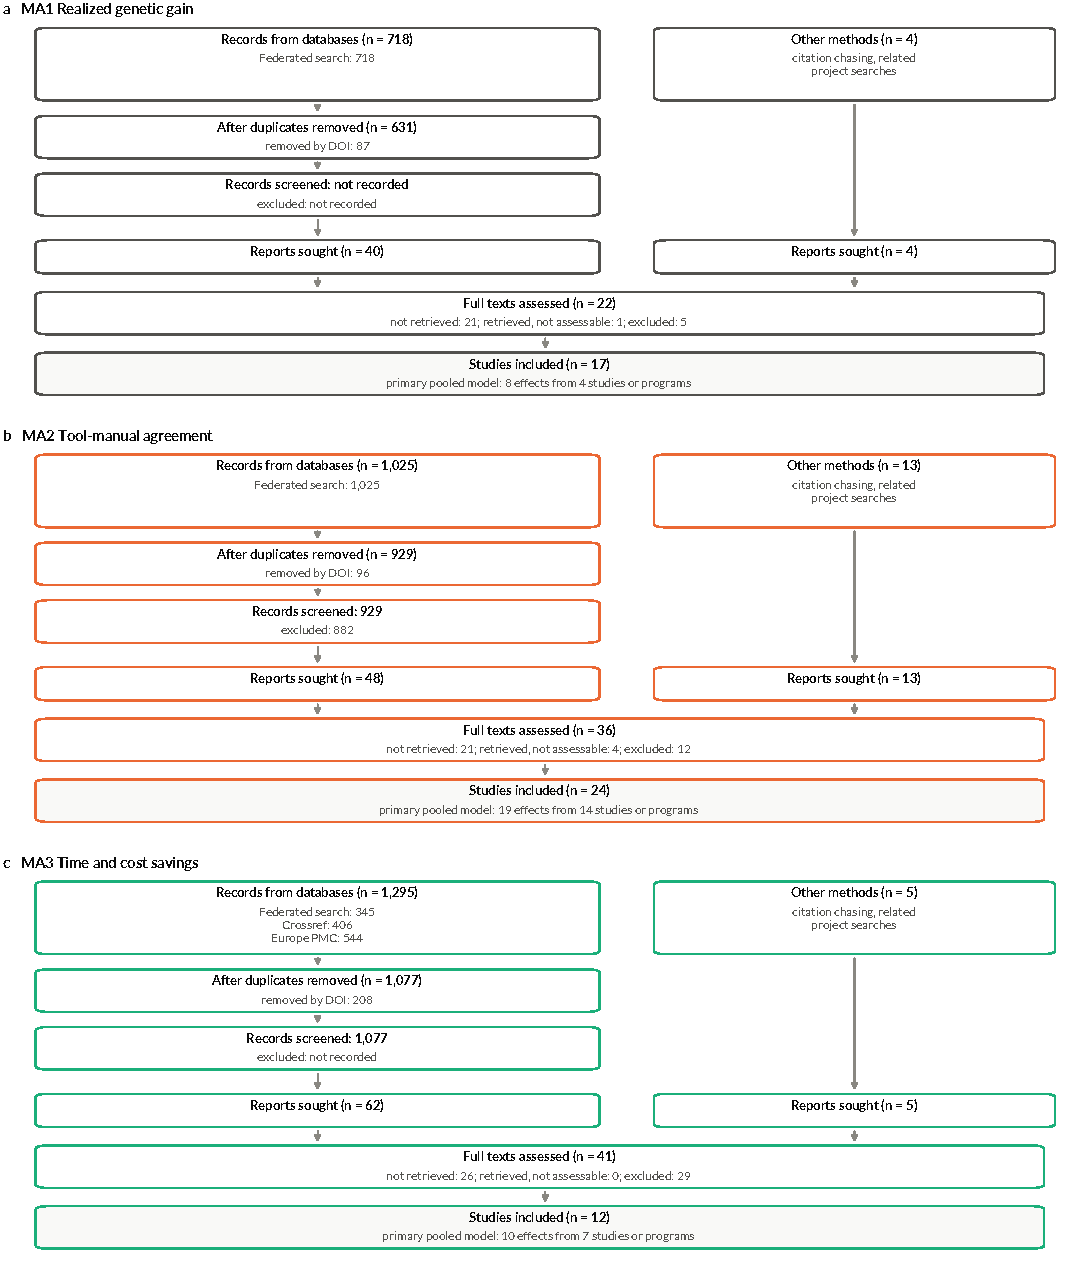
\includegraphics[width=\linewidth]{figS1_prisma.pdf}
\caption{PRISMA 2020-style flow diagrams for (a) MA1 realized genetic gain, (b) MA2 agreement between
image-based or AI tools and manual references and (c) MA3 time and cost savings. Duplicates were removed by
DOI. ``Not recorded'' marks steps for which no record-level log exists. Other methods: candidates found in
reference lists or in the other literature searches of this project.}
\label{fig:S1}
\end{figure}
\end{document}
